\documentclass[11pt]{article}

\usepackage[T1]{fontenc}
\usepackage[polish]{babel}
\usepackage[utf8]{inputenc}
\usepackage{lmodern}
\usepackage{amsfonts}
\usepackage{enumerate}
\usepackage{graphicx}
\usepackage{float}
\usepackage[margin=1in]{geometry}
\usepackage{mathtools}

\selectlanguage{polish}
\graphicspath{{../images/}}

\begin{document}
\title{Sprawozdanie 123}
\author{Jacek Gosztyła, Antoni Mleczko}
\maketitle
\section{Cel ćwiczenia} 
Poznanie własności warstwowych złącz półprzewodnikowych typu p-n. Wyznaczenie charakterystyki stało prądowej różnego rodzaju diod. 
\section{Wstęp teoretyczny}
Ze względu na różnice konduktywności (przewodzenie elektrycznego) możemy podzielić ciała na: 
\begin{itemize}
\item przewodniki - dobrze przewodzą prąd elektryczny
\item półprzewodniki - konduktywność może być zmieniana poprzez domieszkowanie, ogrzewanie i inne czynniki
\item izolatory - nie przewodzą prądu. 
\end{itemize}

Nośniki ładunku w przewodnikach i półprzewodnikach możemy podzielić na elektrony i dziury. \\
Nośniki możemy stworzyć dodając odpowiednie substancje. Dodając akceptory które popierają elektrony, zwiększamy ilość dziur które przy dużej ilości akceptorów stają się nośnikiem większościowym. \\
Żeby zwiększyć liczbą nośników elektronów, musimy użyć  domieszki donorowej - ona dodaje elektrony. \\
W półprzewodniku samoistnym (bez domieszek) koncentracje elektronów n i dziur p są równe. \\
Charakterystyka prądowo napięciowa złącza p - n jest nieliniowa. Dobrze przewodzi w kierunku przewodzenia, natomiast prawie w ogóle nie przewodzi w  kierunku zaporowym.  \\ 
Gdy na końce złącza p-n przyłożymy napięcie w kierunku przewodzenia, dziury będą mogły się swobodnie przemieszczać. W przeciwnym wypadku będą przemieszczać się tylko nośniki mniejszościowe, a więc prąd nie będzie płynął. 


% Kierunek przewodzenia / zaporowy.
% Polaryzacja przewodzenia - 
% Charakterystyka prądowo-napięciowa. 
% Współczynnik idealności.
% Przesunięcie charakterystyk diody krzemowej względem germanowej. 
% Przerwa energetyczna. 
% Określenie materiału z jakiego wykonana jest dioda. 
% Dioda germanowa, dioda Zenera, dioda świecąca. 
% Polaryzacja zaporowa. 
% Napięcie stabilizowane.
% Współczynnik stabilizacji. 

\section{Wykonanie doświadczenia}
W celu wyznaczenia charakterystyk odpowiednich diód, posłużyliśy się układem, którego schemat widoczny jest na Rys.1. w załączonych materiałach. Do pomiaru były cztery rodzaje diód:
\begin{itemize}
    \item{Germanowa - Ge}
    \item{Krzemowa - Si}
    \item{Świecąca - LED}
    \item{Zenera}

W kierunku przewodzenia wyznaczaliśmy napięcie wytwarzane na diodzie w zależności od funkcji płynącego prądu (tj. natężenia).
W kierunku zaporowym jednak, jedynie charakterystyka diody Zenera była wyznaczana jako funkcja napięcia od natężenia. Diody Germanowa, Krzemowa i LED były badane jako funkcja natężenia prądu w zależności od podanego napięcia. Dla diody Germanowej w kierunku zaporowym, zmierzone zostały także bardzo małe napięcia - rzędu $10^{-2}$.
\end{itemize}
\section{Opracowanie wyników pomiarów}
\subsection{Kierunek przewodzenia}
\subsubsection{Wspólny wykres charakterystyk prądowo- napięciowych  }

\begin{figure}[H]
    \centering
    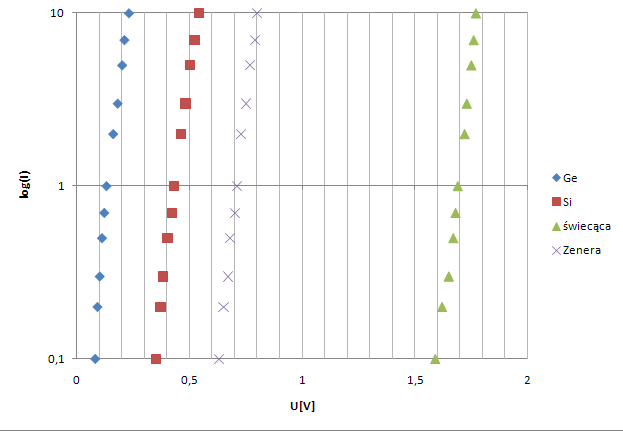
\includegraphics[height=0.27\paperheight]{graph1}
    \label{fig:graph1}
\end{figure}

\subsubsection{Wykres charakterystyki napięciowej dla diody krzemowej. }


\begin{figure}[H]
    \centering
    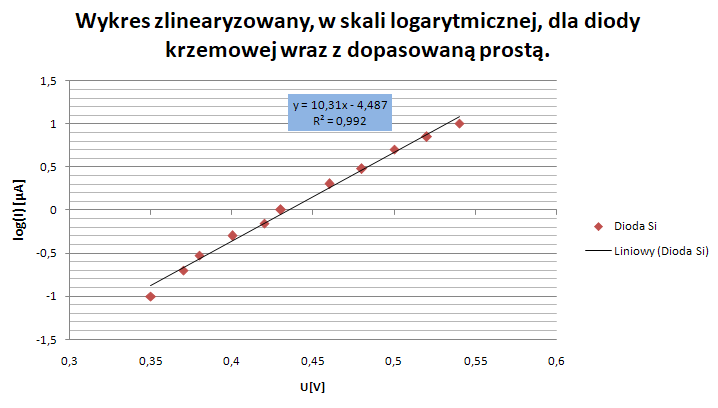
\includegraphics[height=0.27\paperheight]{graph2}
    \label{fig:graph2}
\end{figure}

\subsubsection{Współczynnik idealności dla diody krzemowej. }
Do wyznaczenia współczynnika idealności skorzystamy z zależności prawdziwej dla małych $I$:
$$ ln(I) = ln(I_s) + \frac{e}{mkT}U $$
$$ gdzie \beta =  ln(I_s), \alpha =  \frac{e}{mkT}U $$
Stąd:
$$ m = \frac{1}{\alpha U_t} $$
Przyjmujemy $ U_t = 26mV $.
Korzystając z funkcji REGLINP otrzymujemy $ \alpha = 10,3096$.
Zatem
$$ m = \frac{1}{10,3096*26} =  2,52 $$


\subsubsection{Przesunięcie charakterystyk diody Si i Ge}
Średnia wartość różnicy $U_{Si} - U_{Ge}$ wyniosła: $U_{Si} - U_{Ge} = 0.3V$, taką samą różnicę zaobserwowano także w większości punktów pomiarowych (tzn. jest także medianą).\\
\newline
Wartość przerwy energetycznej dla krzemu wynosi: $W_{gSi} = 1,11eV$\\
Wartość przerwy energetycznej dla germanu wynosi: $W_{gGe} = 0,67eV$\\
Różnica między podanymi wartościami $W_{gSi} - W_{gGe} = 0,44eV$\\
\newline
Widzimy, że różnica napięć pomiędzy dwoma diodami, jest mniejsza niż różnica ich przerw energetycznych (po przedzieleniu jednostki $eV$ przez $1e$), pomimo tego iż w teorii wielkości te powinny być sobie równe. Może to wynikać z niedokładności urządzeń pomiarowych i temperatury (jako, że wartość przerwy enetgetycznej podaje się w temperaturze 300K) 

\subsubsection{Przesunięcie charakterystyk diody Si i LED}
Średnia wartość różnicy $U_{LED} - U_{Si}$ wyniosła: $U_{LED} - U_{Si} = 1.26V$, taką samą różnicę zaobserwowano także w większości punktów pomiarowych (tzn. jest także medianą).\\
\newline
Wartość przerwy energetycznej dla krzemu wynosi: $W_{gSi} = 1,11eV$. Wynika stąd, że:
$$W_{gLED} - W_{gSi} \approx 1.26eV$$
$$W_{gLED} \approx 2.37eV$$
\\
W diodzie LED mamy zależność:
$$\lambda = \frac{hc}{W_{g}}$$
\\
W naszym przypadku zmierzona $\lambda$ wynosi $\lambda \approx 523.85nm$, co odpowiada wartości koloru zielonego i pokrywa się z kolorem diody użytej w eksperymencie.
\subsubsection{Materiał diody Zenera}
Aby wyznaczyć materiał z jakiego wykonana została dioda Zenera, posłyżymy się podobną techniką jak w punktach powyżej. Średnia różnica $U_{Zenera} - U_{Si} = 0.28V$. Wartość przerwy energetycznej dla krzemu wynosi: $W_{gSi} = 1,11eV$. Wynika stąd, że:
$$W_{gZenera} - W_{gSi} \approx 0.28eV$$
$$W_{gZenera} \approx 1.39eV$$
Co najbliższe jest wartości odpowiadającej fosforkowi indu ($1.35eV$) lub arsenkowi galu ($1.43eV$).
\subsection{Kierunek zaporowy}
\subsubsection{Wykresy charakterystyk napięciowych dla diody germanowej,krzemowej, Zenera i diody świecącej. }

\begin{figure}[H]
    \centering
    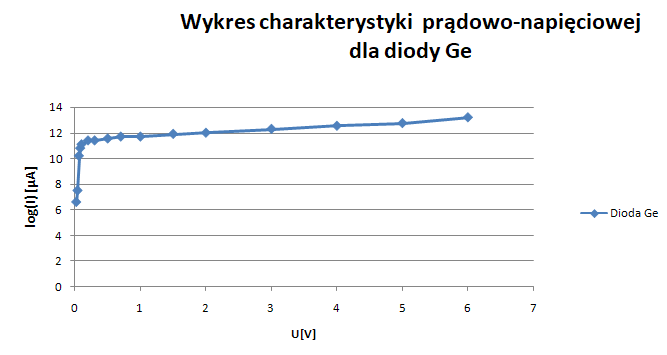
\includegraphics[height=0.27\paperheight]{graph3}
    \label{fig:graph3}
\end{figure}

\begin{figure}[H]
    \centering
    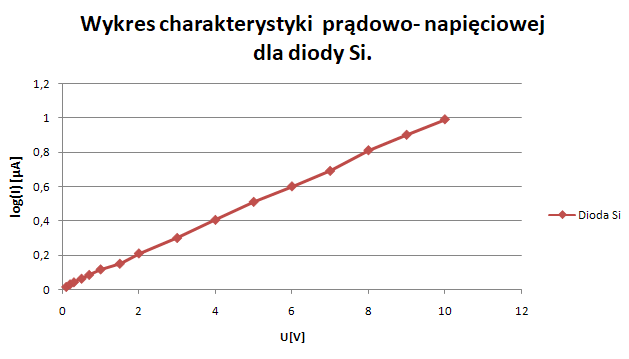
\includegraphics[height=0.27\paperheight]{graph4}
    \label{fig:graph4}
\end{figure}

\begin{figure}[H]
    \centering
    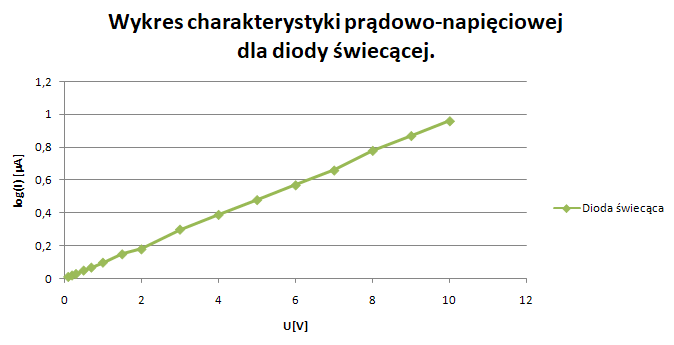
\includegraphics[height=0.27\paperheight]{graph5}
    \label{fig:graph5}
\end{figure}

\begin{figure}[H]
    \centering
    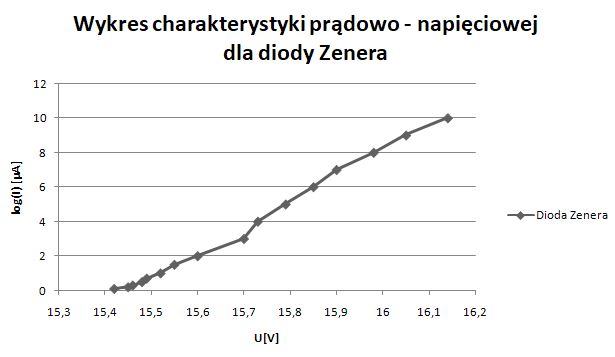
\includegraphics[height=0.27\paperheight]{graph6}
    \label{fig:graph6}
\end{figure}
\subsubsection{Dioda Zenera}
Napięcie stablizowane diody Zenera, odczytane dla warotści $I = 5mA$ wynosi $U = 15.79V$.
Aby obliczyć współczynnik stabilizacji, wyliczamy odpowiednio rezystancję statyczną i dynamiczną. Do wyliczenia $\Delta U$ i $\Delta I$ użyjemy prądów z zakresu $2mA-8mA$:

$$R = \frac{U_{Z}}{I_{0}} = \frac{15.79V}{5mA} = 3158\Omega$$
$$r = \frac{\Delta U}{\Delta I} = \frac{0.38V}{6mA} = 63.3\Omega$$
Współczynnik stabilizacji $Z$ wynosi:
$$Z = \frac{r}{R} \approx 0.02$$ 

\section{Wnioski}
Charakterystyka diód, zgodnie z przewidywaniami wykazała charakter eksponencjalny. W kierunku przewodzenia wszystkie diody wykazują stopniowy wzrost wartości napięcia w zależności od rosnącego natężenia. W kierunku zaporowym, dioda Germanowa wykazuje przy małych napięciach duże skoki prądu w zależności od zmian napięcia. Stabilniejsza okazała się dioda krzemowa i świecąca (która naturalnie, w kierunku zaporowym nie swieciła).
Dioda Zenera spolaryzowana w kierunku zaporowym może być wykorzystywana jako stabilizator napięcia, dzięki temu, iż dużemu zakresowi zmian prądu odpowiadają małe skoki napięcia. W zmierzonym przez nas układzie stosunek względnej zmiany napięcia do względnej zmiany prądu wyniósł zaledwie $0.02 = 2\%$.
\end{document}

